\section{Results}

The experiments were conducted using \texttt{iperf3} with UDP payloads of $L=1472$\,B (i.e., $1472 + 8\,\text{B}_{\text{UDP}} + 20\,\text{B}_{\text{IP}} = 1500$\,B, exactly filling the Ethernet MTU without triggering IP fragmentation) and TCP segments of $L=1460$\,B (i.e., $\text{MTU} - 40$\,B), with a target bitrate of 2\,Gb/s and a test duration of 20\,s per run.

\textbf{Ethernet (baseline).}
Over Ethernet, UDP achieved a stable goodput of $\approx$957\,Mb/s (std.\,dev.\ $<1$\,Mb/s) in both forward and reverse directions, with \textbf{zero datagram loss} on the sender side and only 28 lost datagrams out of 1.6\,M ($\approx$0.002\%) on the receiver in reverse mode. The $\sim$15\,Mb/s gap between UDP and TCP on Ethernet is consistent with the additional overhead of TCP headers and ACK segments, confirming the theoretical formulas: $\mu_{UDP} > \mu_{TCP}$.

\textbf{WiFi--WiFi (UDP).}
When both hosts were connected via WiFi, the results have shown the unreliability of the wireless medium for the UDP traffic:
\begin{itemize}[noitemsep]
    \item \textbf{Forward UDP} average goodput was 180\,Mb/s (std.\,dev.\ 39.78) with values ranging from 130 to 291\,Mb/s. The sender reported 0\% loss, but the receiver recorded \textbf{32\% datagram loss} (97\,857 out of 306\,320). This shows that the sender injected traffic faster than the wireless link could sustain, and since UDP has no flow control, the excess datagrams were dropped.
    \item \textbf{Reverse UDP} average goodput dropped to 106\,Mb/s with \textbf{50\% loss} (182\,701/361\,909 datagrams) and the bitrate ranged from 7.28\,Mb/s to 196\,Mb/s (std.\,dev.\ 67.71). 
\end{itemize}
The differences in performance are attributable to differences in the wireless adapters and the scheduling behaviour of the remote server.

Figure~\ref{fig:wifi-udp-rev-io} shows the I/O graph for the WiFi-WiFi UDP reverse test. The continuous line (received packets) shows a lot of fluctuations, starting the first two seconds near zero, followed by a brief peak around $t=4$\,s, then back to zero before ramping up to $\approx$15\,000\,packets/s between $t=10$--$18$\,s. The dashed line at the bottom represents the negligible traffic in the opposite direction (ACKs are not used in UDP). The shape of the curve confirms that the wireless link alternated between periods of near-total blockage and partial recovery, with no feedback mechanism to regulate the sender.

\begin{figure}[H]
    \centering
    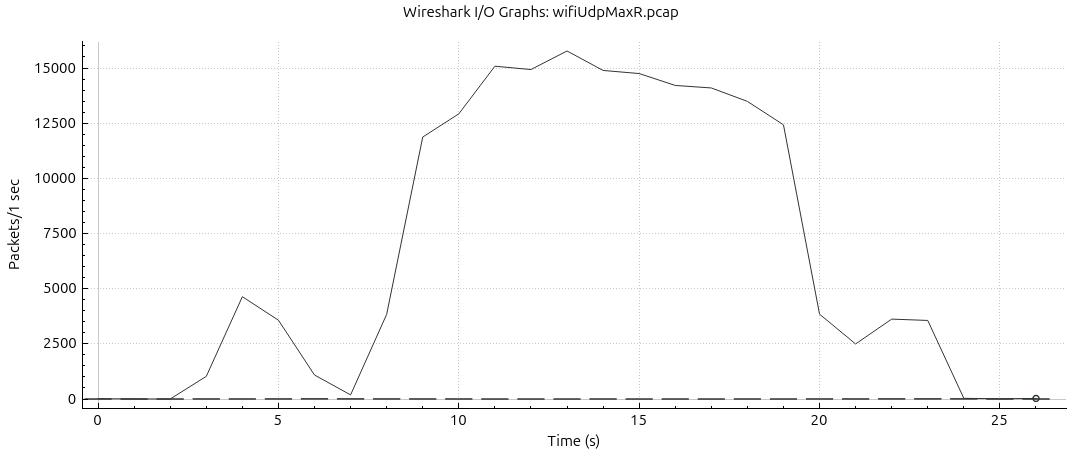
\includegraphics[width=\columnwidth]{imgs/wifiUdpMaxR.jpeg}
    \caption{Wireshark I/O Graph: WiFi--WiFi UDP reverse --- received packet rate oscillates between near-zero and $\approx$15\,000\,pkt/s, reflecting the 50\% overall datagram loss.}
    \label{fig:wifi-udp-rev-io}
\end{figure}

\textbf{WiFi--WiFi (TCP).}
TCP measured lower goodput ($\approx$153\,Mb/s forward, 70\,Mb/s reverse) but achieved \textit{reliable delivery}, through retransmissions. Moreover, the reverse TCP connection dropped to 0\,Mb/s for 6 consecutive seconds (in the interval 15-20\,s), suggesting a link degradation or contention event. TCP's congestion control (Cwnd drops from 1.79\,MB to 1.04\,MB after retransmissions) adapted to these conditions, whereas UDP would simply lose all datagrams during such outages.

Figure~\ref{fig:wifi-tcp-rev-io} shows the I/O graph for the WiFi--WiFi TCP reverse test. The red bars in the bottom represent retransmitted segments, which cluster around $t=10$--$14$\,s, exactly when the throughput curve shows sharp drops. After $t=20$\,s the throughput falls to near zero, corresponding to the 6-second stall observed in the iperf3 output. The contrast with Figure~\ref{fig:wifi-udp-rev-io} is evident: TCP actively adapts its sending rate through congestion control, whereas UDP provides no such mechanism.

\begin{figure}[H]
    \centering
    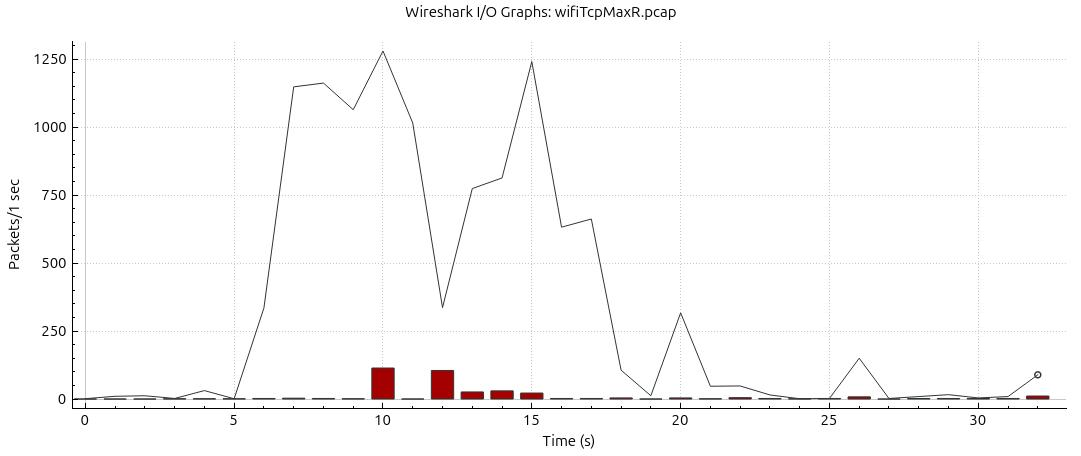
\includegraphics[width=\columnwidth]{imgs/wifiTcpMaxR.jpeg}
    \caption{Wireshark I/O Graph: WiFi--WiFi TCP reverse --- red bars indicate retransmission bursts; the throughput collapses after $t \approx 20$\,s.}
    \label{fig:wifi-tcp-rev-io}
\end{figure}

\textbf{Mixed (WiFi client $\rightarrow$ Ethernet server).}
The mixed scenario produced intermediate results. UDP in the forward direction (WiFi sender, Ethernet receiver) averaged 344\,Mb/s with near-zero loss (5/584\,837, i.e., $< 0.001\%$), indicating that the WiFi uplink was the bottleneck but not saturated to the point of massive loss. However, in \textbf{reverse} mode (Ethernet sender, WiFi receiver), the Ethernet host injected traffic at $\approx$952\,Mb/s while the WiFi interface could only absorb $\approx$208\,Mb/s, resulting in \textbf{78\% datagram loss} (1\,258\,067/1\,610\,724). This is a clear illustration of UDP's lack of flow control: the sender has no mechanism to slow down, and datagrams are silently discarded when the receiver cannot keep up.

Figure~\ref{fig:mix-udp-rev-io} shows the I/O graph for the mixed UDP reverse test, captured at the WiFi receiver. The packet rate peaks at $\approx$27\,000\,pkt/s around $t=10$\,s but shows two troughs---one near $t=8$\,s and another at $t=14$\,s where it drops to $\approx$4\,000\,pkt/s. These troughs correspond to intervals where the WiFi link was temporarily saturated or contending, and since the Ethernet sender has no mechanism to detect this congestion, it continues to transmit at full rate. The datagrams arriving during these periods are silently discarded.

\begin{figure}[H]
    \centering
    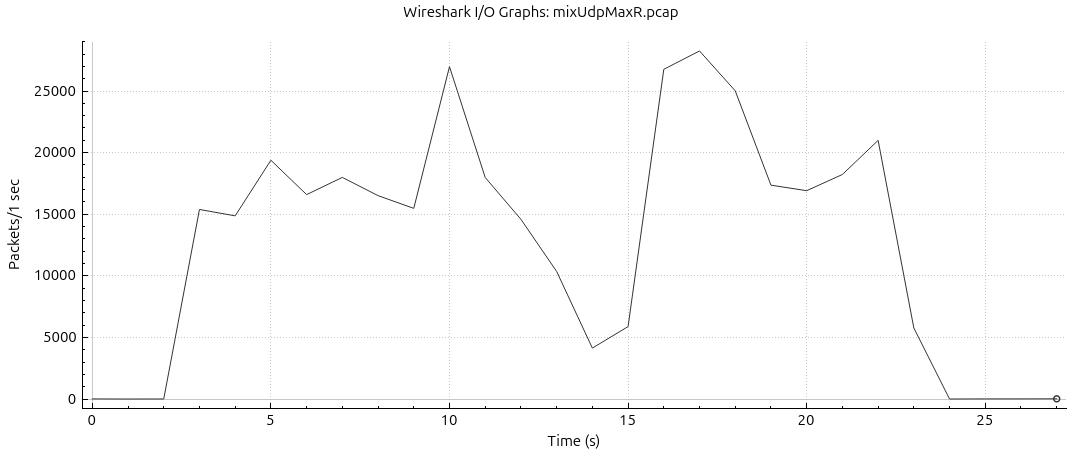
\includegraphics[width=\columnwidth]{imgs/mixUdpMaxR.jpeg}
    \caption{Wireshark I/O Graph: Mixed UDP reverse --- peaks at $\approx$27\,000\,pkt/s with deep troughs, illustrating the 78\% datagram loss caused by the Ethernet--WiFi rate mismatch.}
    \label{fig:mix-udp-rev-io}
\end{figure}